\documentclass[10pt]{beamer}
\usepackage[utf8]{inputenc}
\usepackage{graphicx}
\usepackage {mathtools}
\usepackage{utopia} %font utopia imported
\usepackage{amsmath}




%Allows cmidrule (horizontal lines in tables)
\usepackage{booktabs}

%Allows to control table size relative to page size
\usepackage{adjustbox}

%Real numbers symbol
\usepackage{amssymb}

%Allows colored text
\usepackage{xcolor}

%Allows to justify text and other text formating features
\usepackage{ragged2e}

%Allows floatbarrier
\usepackage{placeins}

%Caption size
\usepackage{caption}

%Use of subfigures
\usepackage{subcaption}

%Allows hl
\usepackage{color}

%Allows hiding table columns
\usepackage{array}
\newcolumntype{H}{>{\setbox0=\hbox\bgroup}c<{\egroup}@{}}

%Allows landscape 
\usepackage{lscape}

%Allows expectation operator 
 
%Allows multirow for tables (some excel2latex tables need it)
\usepackage{multirow}

%Allos dashed lines in tables
\usepackage{arydshln}

%Allows to control spacing
\usepackage{setspace}

%Allows underset and overset
\usepackage{amsmath}
%Allows doublespace
\usepackage{setspace}

%Theorem environment
\usepackage{amsthm}
\newtheorem{proposition}{Proposition}

\usetheme{CambridgeUS}
\usecolortheme{dolphin}

\newenvironment{benumerate}[1]{
    \let\oldItem\item
    \def\item{\addtocounter{enumi}{-2}\oldItem}
    \begin{enumerate}
    \setcounter{enumi}{#1}
    \addtocounter{enumi}{1}
}{
    \end{enumerate}
}
% set colors
\definecolor{myNewColorA}{RGB}{25,25,112}
\definecolor{myNewColorB}{RGB}{25,25,112}
\definecolor{myNewColorC}{RGB}{25,25,112}
\setbeamercolor*{palette primary}{bg=myNewColorC}
\setbeamercolor*{palette secondary}{bg=myNewColorB, fg = white}
\setbeamercolor*{palette tertiary}{bg=myNewColorA, fg = white}
\setbeamercolor*{titlelike}{fg=myNewColorA}
\setbeamercolor*{title}{bg=myNewColorA, fg = white}
\setbeamercolor*{item}{fg=myNewColorA}
\setbeamercolor*{caption name}{fg=myNewColorA}
\usefonttheme{professionalfonts}
\usepackage{natbib}
\usepackage{hyperref}
%------------------------------------------------------------

\setbeamerfont{title}{size=\large}
\setbeamerfont{subtitle}{size=\small}
\setbeamerfont{author}{size=\small}
\setbeamerfont{date}{size=\small}
\setbeamerfont{institute}{size=\small}
\title[]{Figures and tables using Stata.}%主标题
%\subtitle{ }%%副标题
\author[DEAL 2023]{Ricardo Miranda}%%作者

\institute[Duke University]{}
\date[\textcolor{white}{\today} ]
{\today}

%------------------------------------------------------------
%This block of commands puts the table of contents at the 
%beginning of each section and highlights the current section:
%\AtBeginSection[]
%{
%  \begin{frame}
%    \frametitle{Contents}
%    \tableofcontents[currentsection]
%  \end{frame}
%}
\AtBeginSection[]{
  \begin{frame}
  \vfill
  \centering
  \begin{beamercolorbox}[sep=8pt,center,shadow=true,rounded=true]{title}
    \usebeamerfont{title}\insertsectionhead\par%
  \end{beamercolorbox}
  \vfill
  \end{frame}
}
%------------------------------------------------------------

\begin{document}

%The next statement creates the title page.
\frame{\titlepage}

\begin{frame}{How are economic disadvantages transmitted from parents to children?}

There are several studies documenting how wealth is transferred and inherited. But what about poverty and debt? \\
\bigskip
Smythe, A. looks at the change in wealth over a year and shows that children who spend more money on their parents do not experience an increase in wealth.\\
\bigskip
This is done using the fact that at age 62 parents become eligible for social security support.\\
\bigskip
In this lecture we will go beyond the paper's analysis and explore the story in depth. In the process we will use some trick that make figures and tables more readable and compelling.\\
\bigskip
Useful tool for RA's: https://www.ctan.org/pkg/excel2latex
\end{frame}

\begin{frame}{Getting to know your data:}
    Lets start with a very simple exploratory analysis. Just enlist the main variables and report their basic descriptive statistics.\\
    \bigskip
    \begin{itemize}
        \item Summarize: For ovious reasons
        \item For loop: To iterate over variables
        \item Putexcel: To export tables to excel
    \end{itemize}
    \bigskip
    
    Other approaches: esttab, estout, regression only on the constant.
        
\end{frame}

\begin{frame}{Getting to know your data:}

\begin{table}[]
    \begin{adjustbox}{width=.9\textwidth}
    % Table generated by Excel2LaTeX from sheet 'DescriptiveSummaryStats'
\begin{tabular}{rrrrrrrrrrr}
\toprule
          &           &           &           &           &           &           &           &           &           &  \\
\midrule
          &           & \multicolumn{1}{c}{(1)} &           & \multicolumn{1}{c}{(2)} &           & \multicolumn{1}{c}{(3)} &           & \multicolumn{1}{c}{(4)} &           & \multicolumn{1}{c}{(5)} \\
\multicolumn{1}{l}{Variables} &           & \multicolumn{1}{c}{Mean} &           & \multicolumn{1}{c}{Standard deviation} &           & \multicolumn{1}{c}{First quartile} &           & \multicolumn{1}{c}{Median} &           & \multicolumn{1}{c}{Third quartile} \\
\cmidrule{1-1}\cmidrule{3-3}\cmidrule{5-5}\cmidrule{7-7}\cmidrule{9-9}\cmidrule{11-11}          &           &           &           &           &           &           &           &           &           &  \\
\multicolumn{1}{l}{Parent is white} &           & \multicolumn{1}{c}{0.703} &           & \multicolumn{1}{c}{0.457} &           & \multicolumn{1}{c}{0.000} &           & \multicolumn{1}{c}{1.000} &           & \multicolumn{1}{c}{1.000} \\
          &           &           &           &           &           &           &           &           &           &  \\
\multicolumn{1}{l}{Parent's age at birth} &           & \multicolumn{1}{c}{29.465} &           & \multicolumn{1}{c}{6.758} &           & \multicolumn{1}{c}{25.000} &           & \multicolumn{1}{c}{29.000} &           & \multicolumn{1}{c}{33.000} \\
          &           &           &           &           &           &           &           &           &           &  \\
\multicolumn{1}{l}{Parent's years of education} &           & \multicolumn{1}{c}{14.445} &           & \multicolumn{1}{c}{11.916} &           & \multicolumn{1}{c}{12.000} &           & \multicolumn{1}{c}{13.000} &           & \multicolumn{1}{c}{16.000} \\
          &           &           &           &           &           &           &           &           &           &  \\
\multicolumn{1}{l}{Parent's marital status} &           & \multicolumn{1}{c}{2.094} &           & \multicolumn{1}{c}{1.325} &           & \multicolumn{1}{c}{1.000} &           & \multicolumn{1}{c}{1.000} &           & \multicolumn{1}{c}{3.000} \\
          &           &           &           &           &           &           &           &           &           &  \\
\multicolumn{1}{l}{Child's years of education} &           & \multicolumn{1}{c}{15.281} &           & \multicolumn{1}{c}{14.076} &           & \multicolumn{1}{c}{12.000} &           & \multicolumn{1}{c}{14.000} &           & \multicolumn{1}{c}{16.000} \\
          &           &           &           &           &           &           &           &           &           &  \\
\multicolumn{1}{l}{Parent's real income} &           & \multicolumn{1}{c}{78654.284} &           & \multicolumn{1}{c}{103550.241} &           & \multicolumn{1}{c}{26764.282} &           & \multicolumn{1}{c}{53663.594} &           & \multicolumn{1}{c}{99371.141} \\
          &           &           &           &           &           &           &           &           &           &  \\
\multicolumn{1}{l}{Child's real income} &           & \multicolumn{1}{c}{94959.037} &           & \multicolumn{1}{c}{122711.314} &           & \multicolumn{1}{c}{38623.900} &           & \multicolumn{1}{c}{71868.129} &           & \multicolumn{1}{c}{116069.313} \\
\midrule
          &           &           &           &           &           &           &           &           &           &  \\
\bottomrule
\end{tabular}%

    \end{adjustbox}
\end{table}  

\end{frame}

\begin{frame}{Is there a simple story in your data? Is it a clear one?}

    Now lets explore differences in the sample. Is there any simple evidence that suggest what we think its happening? \\
    \bigskip
    \begin{itemize}
            \item Summarize: For ovious reasons
            \item For loop: To iterate over variables
            \item Putexcel: To export tables to excel
            \item Useful trick: Loop over alphabet letters.
    \end{itemize}
    \bigskip
    Other approaches: Regression on indicators, t-tests, graphical approaches (see next slides) 
    
\end{frame}

\begin{frame}{Is there a simple story in your data? Is it a clear one?}

    \begin{adjustbox}{width=.9\textwidth}
    % Table generated by Excel2LaTeX from sheet 'SummaryStats'
\begin{tabular}{lrccccccc}
\toprule
          &           &           &           &           &           &           &           &  \\
Sample    &           & \multicolumn{3}{c}{All}           &           & \multicolumn{3}{c}{Black between 52 and 72} \\
\cmidrule{1-1}\cmidrule{3-5}\cmidrule{7-9}          &           &           &           &           &           &           &           &  \\
Variables &           & \multicolumn{1}{l}{Parent recieved trans.} &           & \multicolumn{1}{l}{Parent not recieved trans.} &           & \multicolumn{1}{l}{Parent recieved trans.} &           & \multicolumn{1}{l}{Parent not recieved trans.} \\
\cmidrule{1-1}\cmidrule{3-3}\cmidrule{5-5}\cmidrule{7-7}\cmidrule{9-9}          &           & (1)       &           & (2)       &           & (3)       &           & (4) \\
\textbf{Parent is white} &           &           &           &           &           &           &           &  \\
Mean      &           & 0.577     &           & 0.712     &           & 0.032     &           & 0.018 \\
Standard deviation &           & 0.494     &           & 0.453     &           & 0.177     &           & 0.132 \\
          &           &           &           &           &           &           &           &  \\
\textbf{Parent's age at birth} &           &           &           &           &           &           &           &  \\
Mean      &           & 29.274    &           & 29.479    &           & 27.879    &           & 28.392 \\
Standard deviation &           & 7.034     &           & 6.738     &           & 7.029     &           & 7.413 \\
          &           &           &           &           &           &           &           &  \\
\textbf{Parent's years of education} &           &           &           &           &           &           &           &  \\
Mean      &           & 13.648    &           & 14.503    &           & 14.446    &           & 14.082 \\
Standard deviation &           & 15.132    &           & 11.645    &           & 16.801    &           & 12.868 \\
          &           &           &           &           &           &           &           &  \\
\textbf{Parent's marital status} &           &           &           &           &           &           &           &  \\
Mean      &           & 2.709     &           & 2.049     &           & 2.827     &           & 2.486 \\
Standard deviation &           & 1.254     &           & 1.319     &           & 1.301     &           & 1.440 \\
          &           &           &           &           &           &           &           &  \\
\textbf{Child's years of education} &           &           &           &           &           &           &           &  \\
Mean      &           & 15.357    &           & 15.275    &           & 14.863    &           & 13.297 \\
Standard deviation &           & 15.191    &           & 13.992    &           & 14.711    &           & 10.759 \\
          &           &           &           &           &           &           &           &  \\
\textbf{Parent's real income} &           &           &           &           &           &           &           &  \\
Mean      &           & 45855.831 &           & 81050.530 &           & 32547.489 &           & 52017.855 \\
Standard deviation &           & 56100.227 &           & 105792.576 &           & 30329.129 &           & 44634.965 \\
          &           &           &           &           &           &           &           &  \\
\textbf{Child's real income} &           &           &           &           &           &           &           &  \\
Mean      &           & 77361.656 &           & 96244.697 &           & 46422.292 &           & 56559.055 \\
Standard deviation &           & 102312.740 &           & 123975.893 &           & 39698.522 &           & 45236.729 \\
\bottomrule
\end{tabular}%

    \end{adjustbox}
    
\end{frame}

\begin{frame}{Are means sufficiently rich? How can we look at the whole population whithout getting lost?}

    We can plot all the observations (if we are willing to look at just a few variables). The story is not always more clear.\\
    \bigskip
    \begin{enumerate}
        \item Scatter: To observe joint distribution
        \item lfit: Graphical regression
        \item Several aesthetic options for the figures.
        \item Are outliers preventing us from looking at the places where the action happens?
    \end{enumerate}
    
    Other approaches: Bar graphs, boxplots. 
    
\end{frame}

\begin{frame}{Are means sufficiently rich? How can we look at the whole population whithout getting lost?}

\begin{figure}[h!]
  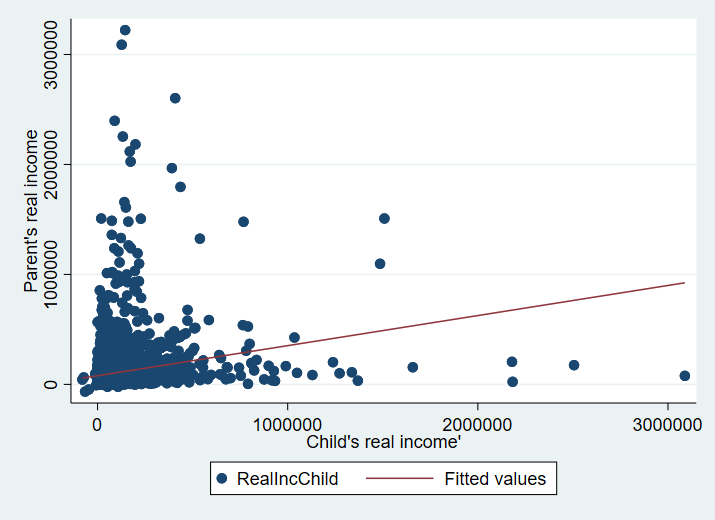
\includegraphics[width=.6\textwidth]{LineFitScatter.png}
\end{figure}%

Are those big numbers messing with the figure?
    
\end{frame}

\begin{frame}{Are means sufficiently rich? How can we look at the whole population whithout getting lost?}

\begin{figure}[h!]
  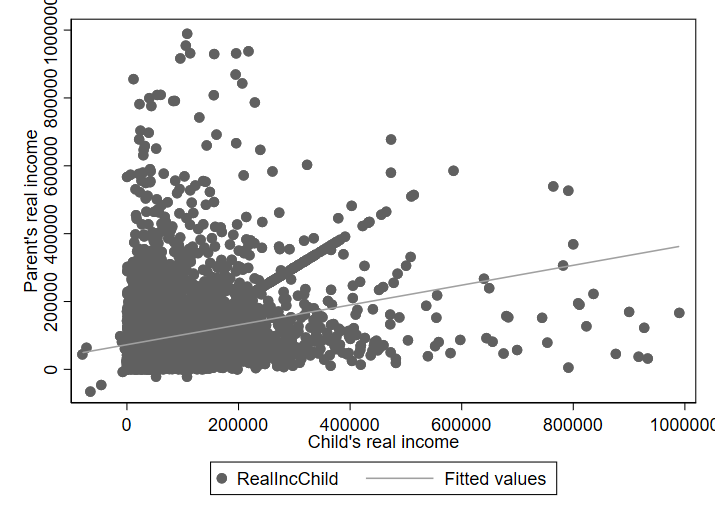
\includegraphics[width=.8\textwidth]{LineFitScatter_Restrict.png}
\end{figure}%

Should we control for covariates?

\end{frame}

\begin{frame}{Are means sufficiently rich? How can we look at the whole population whithout getting lost?}

\begin{figure}[h!]
  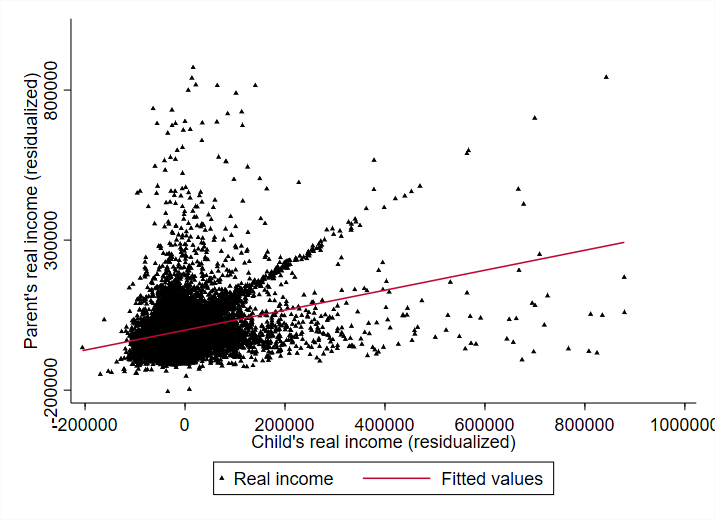
\includegraphics[width=.8\textwidth]{LineFitScatter_Residuals.png}
\end{figure}%
    
\end{frame}

\begin{frame}{A simple but powerful tool: comparing uni-variate densities}

\begin{figure}[h!]
  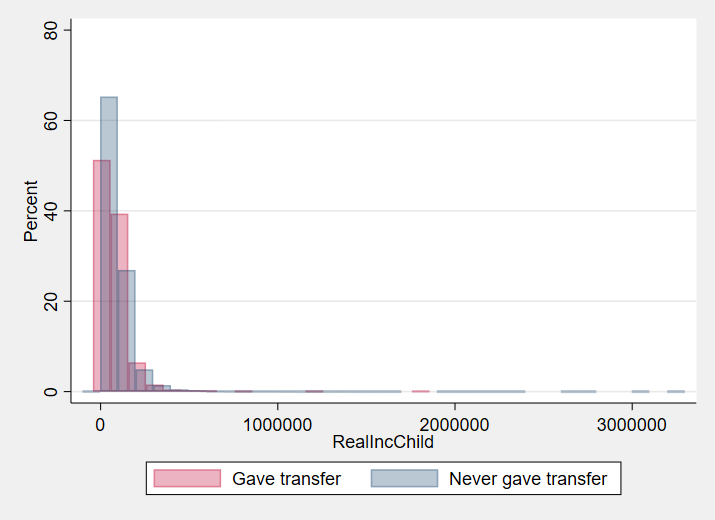
\includegraphics[width=.8\textwidth]{Hist1.png}
\end{figure}%
    
\end{frame}

\begin{frame}{A simple but powerful tool: comparing uni-variate densities}

\begin{figure}[h!]
  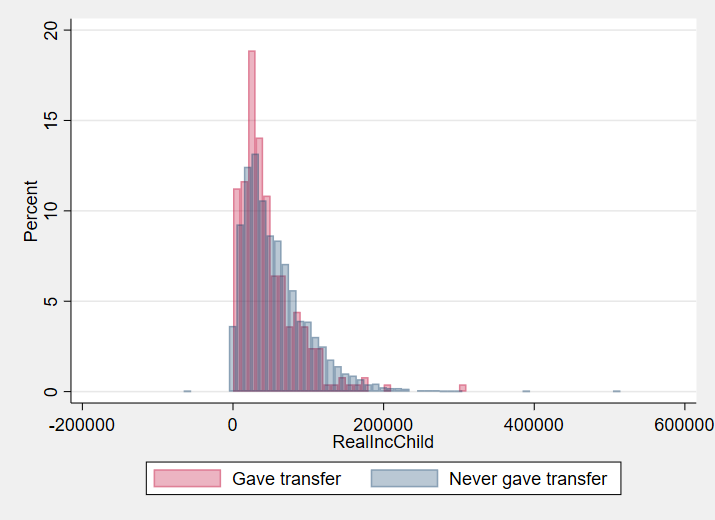
\includegraphics[width=.8\textwidth]{Hist2.png}
\end{figure}%
    
\end{frame}


\begin{frame}{A simple but powerful tool: comparing uni-variate densities}

\begin{figure}[h!]
  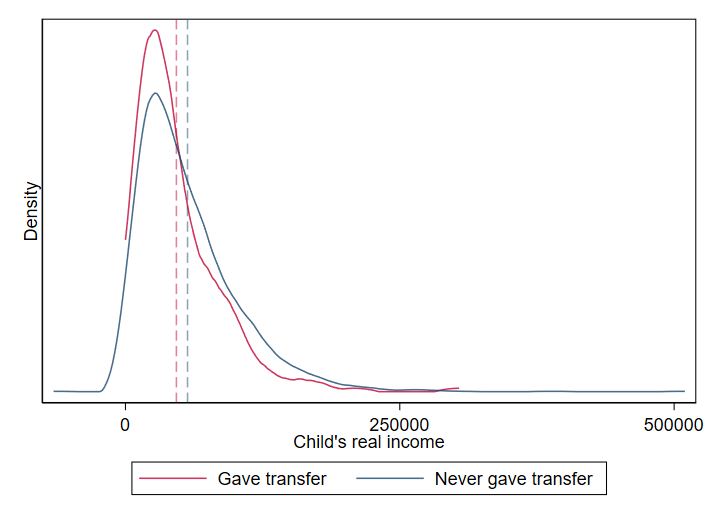
\includegraphics[width=.8\textwidth]{DensityComparison.png}
\end{figure}%
    
\end{frame}

\begin{frame}{Regression analysis}

Do transfers patterns change when parents turn 62?\\
\bigskip
If yes, we can use this change to explore the effect of parents wealth on childrens' wealth.\\
\begin{itemize}
    \item outreg2
    \item Indicators and loops for an organized robustness analysis.
\end{itemize}
\bigskip
Other approaches (for importing results): Loop that writes a latex table, putexcel.

    
\end{frame}

\begin{frame}{Regression analysis}
    \begin{adjustbox}{width=.9\textwidth}
    % Table generated by Excel2LaTeX from sheet 'Regression'
\begin{tabular}{rrrrrrrrrrrrr}
\toprule
          &           &           &           &           &           &           &           &           &           &           &           &  \\
\cmidrule{1-1}\cmidrule{3-4}\cmidrule{6-7}\cmidrule{9-10}\cmidrule{12-13}\multicolumn{1}{c}{\multirow{2}[2]{*}{Variables}} &           & \multicolumn{1}{c}{\multirow{2}[2]{*}{Transfer }} & \multicolumn{1}{c}{\multirow{2}[2]{*}{Wealth change}} &           & \multicolumn{1}{c}{\multirow{2}[2]{*}{Transfer }} & \multicolumn{1}{c}{\multirow{2}[2]{*}{Wealth change}} &           & \multicolumn{1}{c}{\multirow{2}[2]{*}{Transfer }} & \multicolumn{1}{c}{\multirow{2}[2]{*}{Wealth change}} &           & \multicolumn{1}{c}{\multirow{2}[2]{*}{Transfer }} & \multicolumn{1}{c}{\multirow{2}[2]{*}{Wealth change}} \\
          &           &           &           &           &           &           &           &           &           &           &           &  \\
\cmidrule{1-1}\cmidrule{3-4}\cmidrule{6-7}\cmidrule{9-10}\cmidrule{12-13}          &           & \multicolumn{1}{c}{(1)} & \multicolumn{1}{c}{(2)} &           & \multicolumn{1}{c}{(3)} & \multicolumn{1}{c}{(4)} &           & \multicolumn{1}{c}{(5)} & \multicolumn{1}{c}{(6)} &           & \multicolumn{1}{c}{(7)} & \multicolumn{1}{c}{(8)} \\
\multicolumn{1}{l}{Above 62} &           & \multicolumn{1}{c}{-0.0285*} & \multicolumn{1}{c}{10.64*} &           & \multicolumn{1}{c}{-0.0280*} & \multicolumn{1}{c}{11.11*} &           & \multicolumn{1}{c}{-0.0309**} & \multicolumn{1}{c}{11.01*} &           & \multicolumn{1}{c}{-0.0785***} & \multicolumn{1}{c}{10.72*} \\
          &           & \multicolumn{1}{c}{(0.0147)} & \multicolumn{1}{c}{(5.878)} &           & \multicolumn{1}{c}{(0.0149)} & \multicolumn{1}{c}{(6.574)} &           & \multicolumn{1}{c}{(0.0150)} & \multicolumn{1}{c}{(6.400)} &           & \multicolumn{1}{c}{(0.0190)} & \multicolumn{1}{c}{(6.494)} \\
          &           &           &           &           &           &           &           &           &           &           &           &  \\
\multicolumn{1}{l}{Parent is black} &           & \multicolumn{1}{c}{} & \multicolumn{1}{c}{} &           & \multicolumn{1}{c}{0.0228} & \multicolumn{1}{c}{10.14} &           & \multicolumn{1}{c}{0.0227} & \multicolumn{1}{c}{9.971} &           & \multicolumn{1}{c}{0.0318*} & \multicolumn{1}{c}{9.286} \\
          &           & \multicolumn{1}{c}{} & \multicolumn{1}{c}{} &           & \multicolumn{1}{c}{(0.0157)} & \multicolumn{1}{c}{(8.420)} &           & \multicolumn{1}{c}{(0.0158)} & \multicolumn{1}{c}{(8.283)} &           & \multicolumn{1}{c}{(0.0164)} & \multicolumn{1}{c}{(8.326)} \\
          &           &           &           &           &           &           &           &           &           &           &           &  \\
\multicolumn{1}{l}{Female child} &           & \multicolumn{1}{c}{} & \multicolumn{1}{c}{} &           & \multicolumn{1}{c}{-0.0294*} & \multicolumn{1}{c}{-10.93*} &           & \multicolumn{1}{c}{-0.0279*} & \multicolumn{1}{c}{-10.99*} &           & \multicolumn{1}{c}{-0.0241} & \multicolumn{1}{c}{-9.675*} \\
          &           & \multicolumn{1}{c}{} & \multicolumn{1}{c}{} &           & \multicolumn{1}{c}{(0.0153)} & \multicolumn{1}{c}{(6.070)} &           & \multicolumn{1}{c}{(0.0153)} & \multicolumn{1}{c}{(6.072)} &           & \multicolumn{1}{c}{(0.0157)} & \multicolumn{1}{c}{(5.355)} \\
          &           &           &           &           &           &           &           &           &           &           &           &  \\
\cmidrule{1-1}\cmidrule{3-4}\cmidrule{6-7}\cmidrule{9-10}\cmidrule{12-13}\multicolumn{1}{l}{Included variables} &           &           &           &           &           &           &           &           &           &           &           &  \\
\multicolumn{1}{l}{Parent 'syears of educ.} &           &           &           &           & \multicolumn{1}{c}{Yes} & \multicolumn{1}{c}{Yes} &           & \multicolumn{1}{c}{Yes} & \multicolumn{1}{c}{Yes} &           & \multicolumn{1}{c}{Yes} & \multicolumn{1}{c}{Yes} \\
          &           &           &           &           &           &           &           &           &           &           &           &  \\
\multicolumn{1}{l}{Child's years of educ} &           &           &           &           &           &           &           & \multicolumn{1}{c}{Yes} & \multicolumn{1}{c}{Yes} &           & \multicolumn{1}{c}{Yes} & \multicolumn{1}{c}{Yes} \\
          &           &           &           &           &           &           &           &           &           &           &           &  \\
\multicolumn{1}{l}{Parent's age} &           &           &           &           &           &           &           &           &           &           & \multicolumn{1}{c}{Yes} & \multicolumn{1}{c}{Yes} \\
          &           &           &           &           &           &           &           &           &           &           &           &  \\
\multicolumn{1}{l}{Child's age} &           &           &           &           &           &           &           &           &           &           & \multicolumn{1}{c}{Yes} & \multicolumn{1}{c}{Yes} \\
          &           &           &           &           &           &           &           &           &           &           &           &  \\
\multicolumn{1}{l}{Dep. Var mean.} &           & \multicolumn{1}{c}{0.0591} & \multicolumn{1}{c}{13.42} &           & \multicolumn{1}{c}{0.0591} & \multicolumn{1}{c}{13.42} &           & \multicolumn{1}{c}{0.0591} & \multicolumn{1}{c}{13.42} &           & \multicolumn{1}{c}{0.0591} & \multicolumn{1}{c}{13.42} \\
          &           &           &           &           &           &           &           &           &           &           &           &  \\
\multicolumn{1}{l}{R-squared} &           & \multicolumn{1}{c}{0.002} & \multicolumn{1}{c}{0.002} &           & \multicolumn{1}{c}{0.005} & \multicolumn{1}{c}{0.004} &           & \multicolumn{1}{c}{0.008} & \multicolumn{1}{c}{0.005} &           & \multicolumn{1}{c}{0.018} & \multicolumn{1}{c}{0.005} \\
          &           &           &           &           &           &           &           &           &           &           &           &  \\
\multicolumn{1}{l}{Observations} &           & \multicolumn{1}{c}{1,797} & \multicolumn{1}{c}{1,797} &           & \multicolumn{1}{c}{1,797} & \multicolumn{1}{c}{1,797} &           & \multicolumn{1}{c}{1,797} & \multicolumn{1}{c}{1,797} &           & \multicolumn{1}{c}{1,797} & \multicolumn{1}{c}{1,797} \\
\cmidrule{1-1}\cmidrule{3-4}\cmidrule{6-7}\cmidrule{9-10}\cmidrule{12-13}          &           &           &           &           &           &           &           &           &           &           &           &  \\
\bottomrule
\end{tabular}%

    \end{adjustbox}
    
\end{frame}

\begin{frame}{Regression analysis: Richer patterns}

We can look at how the effect evolves as parents age. 

\begin{figure}[h!]
\begin{subfigure}[t]{.48\textwidth}
  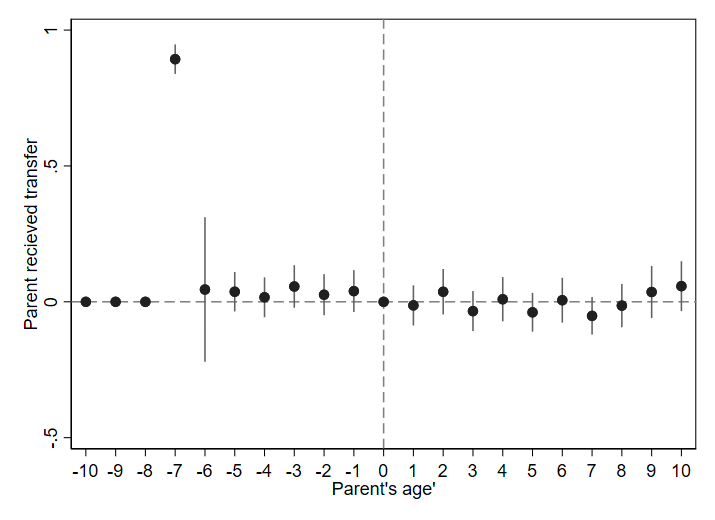
\includegraphics[width=\textwidth]{OLS_Transfer.png}
\end{subfigure}%
\hfill
\begin{subfigure}[t]{.48\textwidth}
  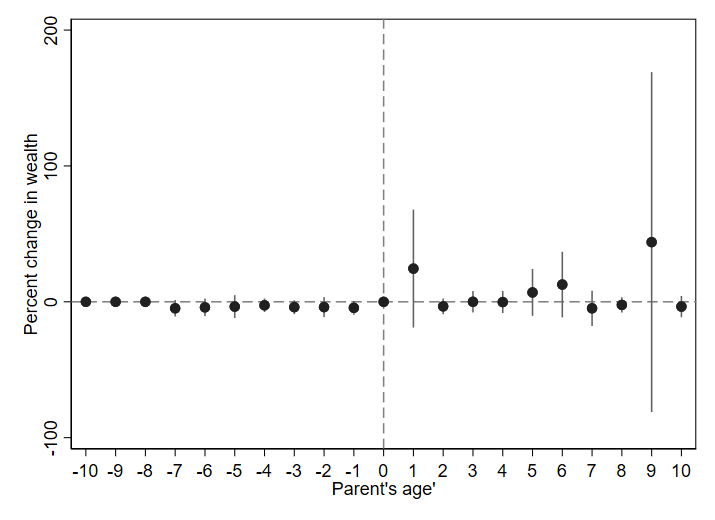
\includegraphics[width=\textwidth]{OLS_ChangeWealth.png}
\end{subfigure}%
\end{figure}%
    
\end{frame}


\begin{frame}{A bit beyond regression analysis: Regression discontinuity}

We can look at how the effect evolves as parents age in an even more flexible way. 

\begin{figure}[h!]
\begin{subfigure}[t]{.48\textwidth}
  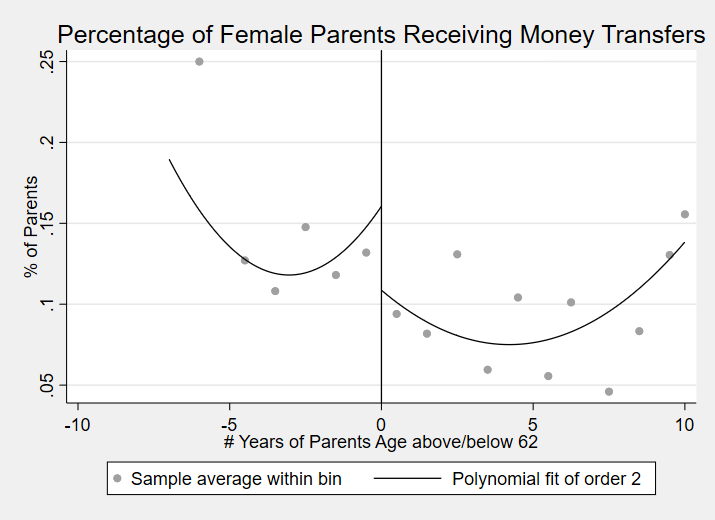
\includegraphics[width=\textwidth]{RD_Transfer.png}
\end{subfigure}%
\hfill
\begin{subfigure}[t]{.48\textwidth}
  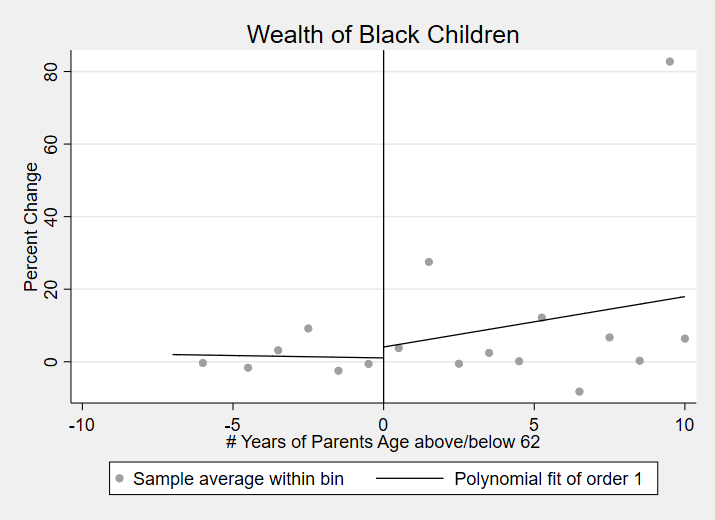
\includegraphics[width=\textwidth]{RD_ChangeWealth.png}
\end{subfigure}%
\end{figure}%
    
\end{frame}

\begin{frame}{Refference:}

Smythe, A. (2022, May). Child-to-Parent Intergenerational Transfers, Social Security, and Child Wealth Building. In AEA Papers and Proceedings (Vol. 112, pp. 53-57). 2014 Broadway, Suite 305, Nashville, TN 37203: American Economic Association.
    
\end{frame}
\end{document}


